\section{Implementierung}

In diesem Kapitel wird die Implementierung des Projektes mit Fokussierung auf die einzelnen Komponenten beschrieben.

\subsection{Kommunikation}

Die Kommunikation der einzelnen Komponenten des Schwarmverhaltens baut auf einer klar definierten Struktur, um ein verteiltes System zu ermöglichen, siehe Abbildung \ref{fig:full_classdiagram}. Die Daten werden dabei als \gls{json} Objekte zur optimalen plattformübergreifenden Interpretation versendet, wobei jeweils die entsprechende Bibliothek zur Serialisierung verwendet wird.
\begin{verbatim}
\end{verbatim}
\begin{figure}[h]
	\begin{center}
		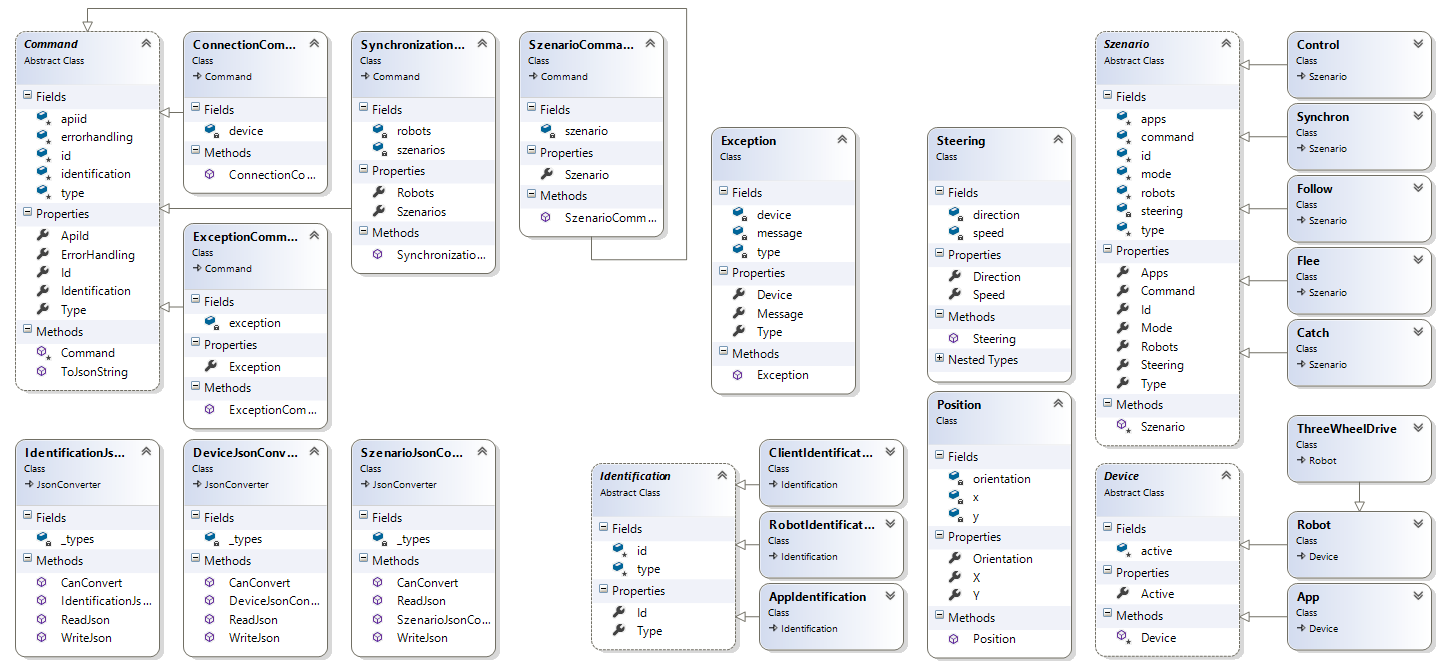
\includegraphics[width=0.95\textwidth]{images/uml/full_class_diagram.png}
	\end{center}
	\caption{Aufbau Commands}
	\label{fig:full_classdiagram}
\end{figure}

\newpage
\noindent
Der Kern zur Implementierung der Kommunikation erfolgt in zwei Methoden, die auf jeder Komponente zur Verfügung stehen. Diese dienen zum Versenden, sowie Empfangen von Daten, wobei diese als Zeichenkette serialisiert und in Bytes aufgeteilt werden, siehe Abbildung \ref{fig:SendCommand}. Um den vollständigen Umfang der Daten zu erfassen, wird die Größe ermittelt und standardmäßig mittels vier Bytes übertragen. Dadurch ist eine maximale Paketgröße von 32 Byte möglich, was einer Länge von etwa 4 Milliarden Zeichen entspricht. Die Interpretation zum Empfangen erfolgt mit ähnlichem Muster, indem zunächst die Größe der Daten festgestellt wird und die Daten deserialiert werden, siehe Abbildung \ref{fig:ReceiveCommand}.

\begin{figure}[h]
	\centering
	\subfloat[Versende Kommando]{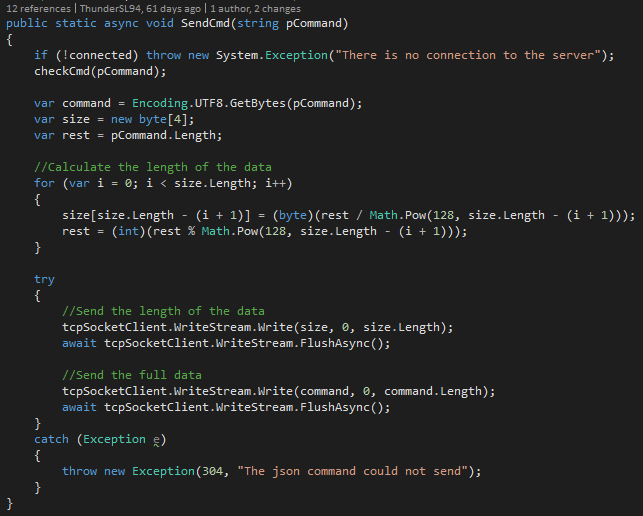
\includegraphics[width=0.6\textwidth]{images/code/SendCommand.png}\label{fig:SendCommand}}
	\qquad
	\subfloat[Empfange Kommando]{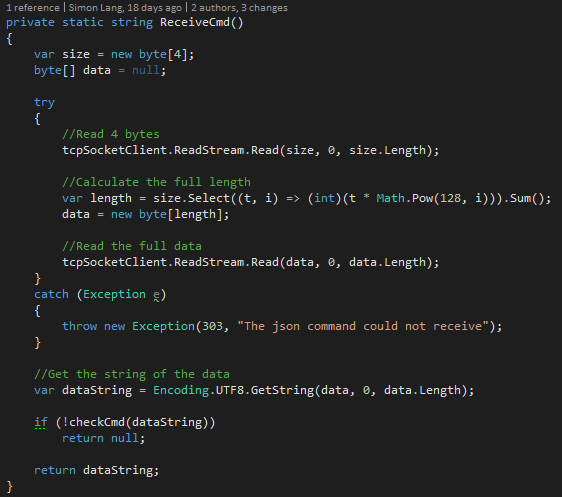
\includegraphics[width=0.6\textwidth]{images/code/ReceiveCommand.png}\label{fig:ReceiveCommand}}
	\caption{Kommunikation}
\end{figure}

\newpage
\paragraph{Kommandos}

\begin{wrapfigure}{r}{0.55\textwidth}
	\begin{center}
		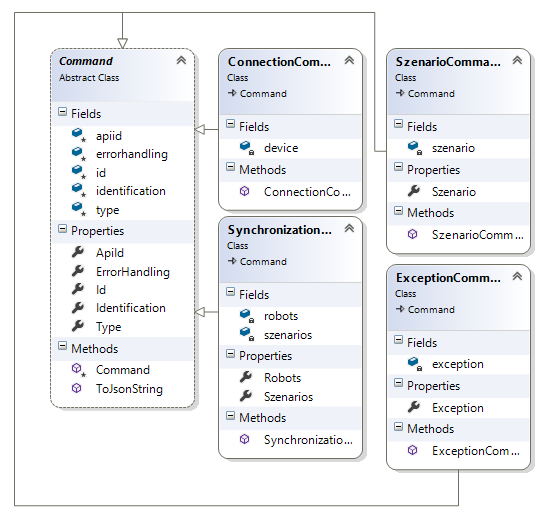
\includegraphics[width=0.5\textwidth]{images/uml/commands.png}
	\end{center}
	\caption{Kommandos}
	\label{fig:commands_classdiagram}
	\begin{center}
		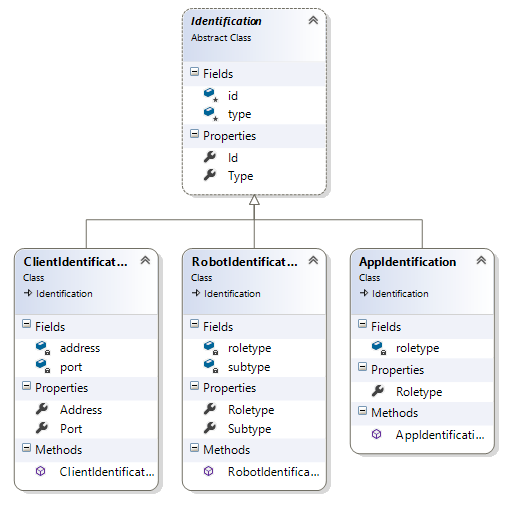
\includegraphics[width=0.5\textwidth]{images/uml/identification.png}
	\end{center}
	\caption{Identifikation}
	\label{fig:identification_classdiagram}
\end{wrapfigure}

stellen die Basis der Kommunikationsstruktur sowie den aktuellen Kontext dar, indem sich die Software befindet, siehe Abbildung \ref{fig:commands_classdiagram}. Sie enthalten grundlegende Attribute zur allgemeinen Identifikation des Kommandos, die zur Interpretation verwendet, welche über definierte Enums ausgewählt werden. Je nach Kommando sind zusätzliche Objekte enthalten, die durch die jeweilige Id vordefiniert sind.\\

\paragraph{Identifikationen}

stellt die individuelle Identität der einzelnen Komponente dar, siehe Abbildung \ref{fig:identification_classdiagram}. Diese wird durch eine fortlaufende Identifikationsnummer, Typen und je nach Ableitung weiteren Attributen erreicht. Um die jeweiligen Kommandos entsprechend zuzuordnen, sind diese in jedem Kommando vorhanden und bilden die Basisobjekte. Die unterschiedlichen Typen sind dabei für verschiedene Kontexte der Software zuständig. Die ClientIdentification stellt einerseits die Verbindung einer allgemeinen Komponente zur Desktopanwendung dar, wogegen die Robot- bzw. AppIdentification die spezifische Identifikation der Komponente darstellt. Die Erstellung der Identifikation erfolgt wiederholt zur Anmeldung der Komponente am System. Zunächst wird ein leeres Objekt erzeugt, dass anschließend durch abfragende Kommandos an die entsprechende Komponente befüllt wird, welche hinterher eine berechnete Identifikationsnummer erhält.

\newpage
\paragraph{Geräte}

\begin{wrapfigure}{r}{0.55\textwidth}
	\begin{center}
		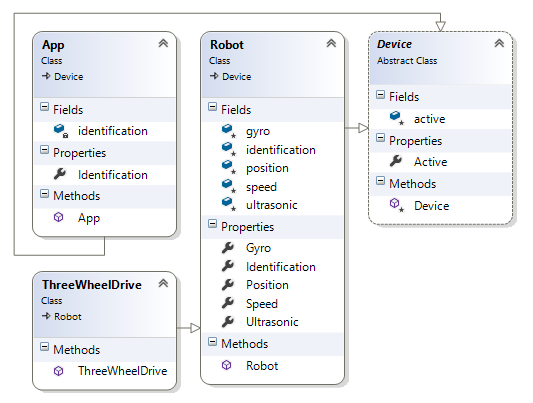
\includegraphics[width=0.5\textwidth]{images/uml/devices.png}
	\end{center}
	\caption{Devices}
	\label{fig:devices_classdiagram}
	\begin{center}
		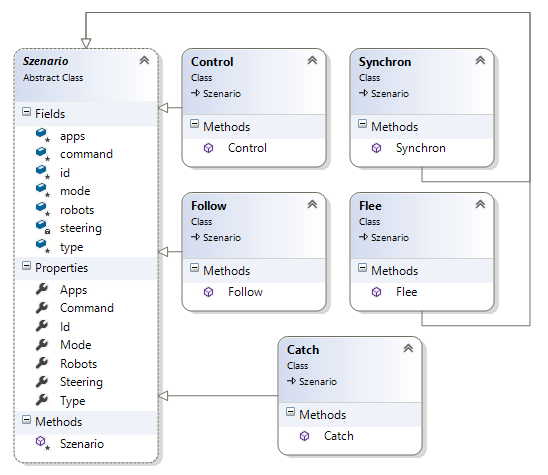
\includegraphics[width=0.5\textwidth]{images/uml/szenarios.png}
	\end{center}
	\caption{Scenarios}
	\label{fig:szenarios_classdiagram}
\end{wrapfigure}

stellen die Komponenten dar, die an einem Szenario eines Schwarmverhaltens teilnehmen, siehe Abbildung \ref{fig:devices_classdiagram}. Sie enthalten jeweils spezifische Identifikations Objekte, zur gegenseitigen Zuordnung, sowie die erfassten Daten der entsprechenden Systeme. Die Unterscheidung erfolgt in zwei Komponenten, dem Robot und der App, wobei der Roboter in die jeweiligen Untertypen gegliedert werden kann. 

\paragraph{Szenarios}

stellen den Ablauf des Schwarmverhaltens dar, in dem sich der Nutzer befindet, siehe Abbildung \ref{fig:szenarios_classdiagram}. Sie enthalten die jeweiligen Teilnehmer des Szenarios, sowie die Steuerungsinformationen und damit die gesamten Daten des aktuellen Kontextes. Diese Objekte werden laufend aktualisiert und besitzen lediglich zur Laufzeit des Szenarios ihre Gültigkeit. Dabei existieren verschiedene Kategorien von Szenarien, siehe Abschnitt \ref{szenarien}. Diese definieren jeweils einen unterschiedlichen Kontext und besitzen daher je nach Szenario zusätzliche Attribute.

\newpage
\paragraph{Konverter}

\begin{wrapfigure}{r}{0.55\textwidth}
	\begin{center}
		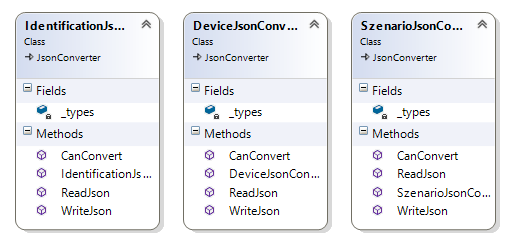
\includegraphics[width=0.5\textwidth]{images/uml/json_converter.png}
	\end{center}
	\caption{JsonConverter}
	\label{fig:converter_classdiagram}
\end{wrapfigure}

dienen der Deserialisierung von abstrakten \gls{json} Objekten, welche nicht direkt identifiziert werden können, siehe Abbildung \ref{fig:converter_classdiagram}. Dazu gehören abstrakte Klassen, sowie Schnittstellen, welche keinem spezifischen Objekt zugeordnet werden kann. Die Implementierung erfolgt durch die Überschreibung der entsprechenden Methoden zur Deserialisierung und Serialisierung, siehe Abbildung \ref{fig:ConverterRead} und \ref{fig:ConverterWrite}. Je nach Anwendung, wird ein Parameter übergeben, der das Objekt als Zeichenkette beinhaltet. Dieses wird durch eine Abfolge von Bedingungen auf den Typen geprüft wird, um das Objekt zu erstellen.\\

\begin{figure}[h]
	\centering
	\subfloat[ReadJson]{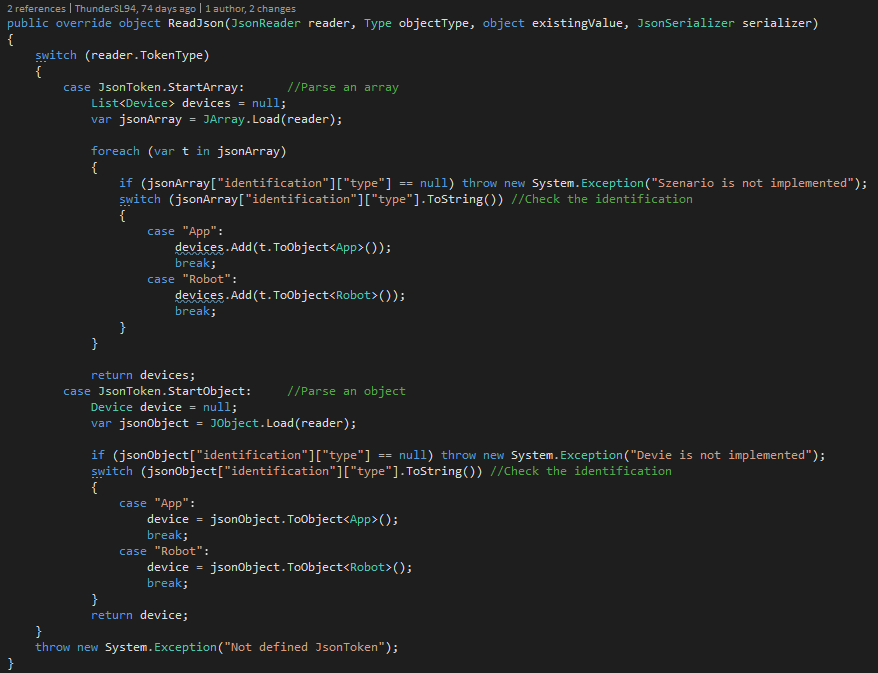
\includegraphics[width=0.6\textwidth]{images/code/DeviceConverterRead.png}\label{fig:ConverterRead}}
	\qquad
	\subfloat[WriteJson]{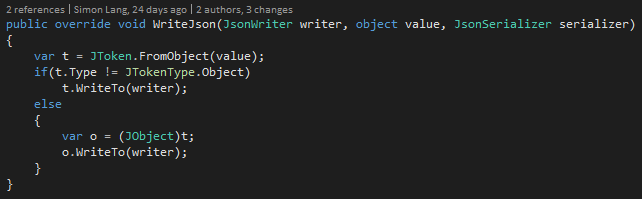
\includegraphics[width=0.6\textwidth]{images/code/DeviceConverterWrite.png}\label{fig:ConverterWrite}}
	\caption{Device JsonConverter}
\end{figure}

\newpage
\subsection{\gls{app}}

Die Erstellung der App erfolgt in einer plattformübergreifenden Implementierung durch Xamarin in C\#. Kernelemente stellen hierbei die Struktur, Oberfläche, Businesslogik sowie das Kommunikationssystem dar. Durch die zentrale Verwendung des Kommunikationssystems wird dieses in ein separates Projekt untergliedert, siehe Abbildung \ref{fig:solution} und wird als solches von der \gls{app} als Bibliothek eingebunden. Somit lässt sich die Logik einmalig implementieren und kann auf andere Systemen entsprechend übertragen werden.\\
Die \gls{app} setzt sich aus vier verschiedenen Projekten zusammen, einer \acrshort{pcl} als Projekt zur plattformübergreifenden Entwicklung und den plattformspezifischen Projekten. Diese werden dem Zielsystem entsprechend ausgewählt und erzeugen durch ihre bestehende Referenz auf die \acrshort{pcl} einen plattformspezifischen Quellcode als \gls{il}, der anschließend ausgeführt werden kann.\\

\begin{figure}[h]
	\begin{center}
		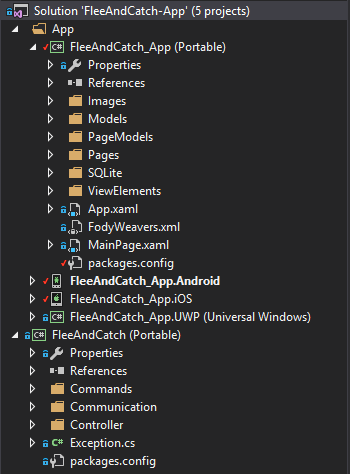
\includegraphics[width=0.5\textwidth]{images/implementation/solution.png}
	\end{center}
	\caption{Projektstruktur}
	\label{fig:solution}
\end{figure}

\newpage
\subsubsection{Workflow} %Struktur

Die Struktur der \gls{app} basiert auf dem in Xamarin verbreiteten Design Pattern \acrlong{mvvm}, welches durch ein Benachrichtigungssystem zwischen den verschiedenen Strukturen der \gls{app} eine Abspaltung der Daten, \gls{gui} und dem Businesscode erlaubt. Zusätzlich wird die standardmäßig vorhandene CodeBehind Struktur der einzelnen Seiten verwendet, wobei der Businesscode an das Layout der Seite gebunden ist, um diese miteinander zu verbinden. Zur lokalen Speicherung der Daten wird SQLite durch eine implementierte Schnittstelle verwendet, welche plattformübergreifend ansprechbar ist.

\paragraph{\acrfull{mvvm}}

stellt ein Design Pattern dar, welches eine grundlegende Struktur im Quellcode ermöglicht, siehe Abbildung \ref{fig:mvvm}. Dabei wird die erstellte Benutzeroberfläche von der Logik, sowie den Daten getrennt, um Änderungen unabhängig voneinander durchführen zu können. Die einzelnen Objekte werden dabei durch Referenzen verbunden um diese durch Events entsprechend zu aktualisieren.\\

\begin{tabular}{p{2.5cm} p{12.25cm}}
	\textbf{Model:} & Datenschicht, welche durch den Benutzer über die \gls{gui} verändert werden kann und über Datenänderungen die entsprechenden Elemente benachrichtigt \\
	\textbf{View:} & \gls{gui} mit den anzuzeigenden Elementen, welche an das ViewModel gebunden sind und der Benutzerinteraktion dienen. \\
	\textbf{ViewModel:} & Logik des \gls{ui} als zentrale Schnittstelle zwischen dem Model und der View zum Austausch von Informationen, indem entsprechende Methoden und Dienste ausgeführt werden. \\
\end{tabular}

\bigskip

\begin{figure}[h]
	\begin{center}
		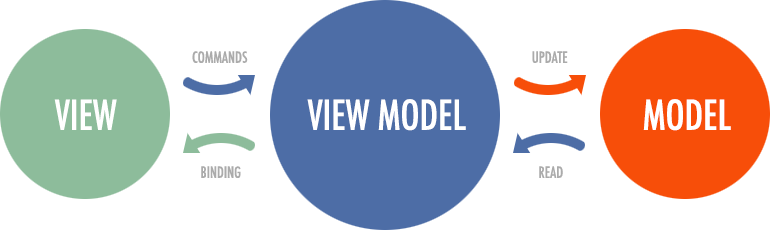
\includegraphics[width=0.95\textwidth]{images/implementation/mvvm.png}
	\end{center}	
	\caption{\acrlong{mvvm} \cite{Brecht.MVVMEntity}}
	\label{fig:mvvm}
\end{figure}

\newpage
\subsubsection{\acrfull{gui}} %Oberfläche

Die Oberfläche der \gls{app} wird mittels \gls{xaml} durch verschiedene von Xamarin zur Verfügung gestellten Elementen realisiert. Da eine \gls{app} ein einfaches Bedienkonzept voraussetzt, damit es von jedem beliebigen Benutzer verwendet werden kann,


Dabei wird für das Layout der einzelnen Seiten vor allem auf ein StackLayout gesetzt. Dieses ist sehr einfach umzusetzen, indem eine Orientierung zur Anordnung der verschiedenen Elemente festgelegt wird, welche anschließend nacheinander eingefügt werden. 




 Dabei wird für die Navigation der einzelnen Seiten vor allem auf die Verwendung der NavigationPage sowie zur Auswahl des Szenarios auf ein Carousel gesetzt. 




 mit den Aufbau eines STacks durch pushund pop aufrufe die entsprechenden Seiten gewechselt werden, siehe Abbildung xx. 

\begin{comment}
	Die Oberfläche der \gls{app} wird mittels \gls{xaml} realisiert. Dabei werden die einzelnen Elemente untereinander in der typischen \gls{xml} Struktur angeordnet und stellen damit die \gls{gui} dar, welche die einzelnen Elemente zur Benutzerinteraktion beinhaltet. Zur Strukturierung des Design bietet Xamarin verschiedene Arten von Layouts, wobei diese \gls{app} auf die Stacklayout zur Struktureirung und einer NavigationPage zur Naviagtion, sowie einem Carousel der Szenario auswahl setzt.
\end{comment}

\begin{comment}
	Die Oberfläche der \gls{app} wird mittels XAML erstellt, welche auf der Basis von XML ist. Dabei werden die einzelnen ELemente untereinnander Strukturuert, wobei der ENtwickler in Xamarin verschiedene Möglichkeiten des Designs besitzt. Grundlegend ist die entscheidung, ob eine plattformspezifisches Design sinnn macht, oder aber ein plattformübergreifendes, wobei dieses weniger Freiheiten bietet. Die plattformübergreifendes Design besitzt eine Reihe von grundlegeneden Layouts, die für Xamamrin eingesetzt werden können, sowie unterschiedliche Seitenarten. Views
	Seiten (ContentPage, MasterDetailPage, NavigationPage, TabbedPage, TemplatedPage, CaruselPage)
	View (ContentPresenter, ContentVIew, ScrollVIew, Frame, TemplatedVIew)
	Layout (Stacklayout, absolutLayout, RelativeLayout, GridLayout)
	
	Weitere standardelemente
	
	Durch verschiednene Packages könenn dabei viele Zusätzliche DInge erstellt werden
\end{comment}


%General, XAML stuff

\begin{figure}[h]
	\begin{center}
		
\includegraphics[width=0.75\textwidth]{images/implementation/push.png}
	\end{center}	
	\caption{Wechsel auf neue Seite}
	\label{fig:push}
	\begin{center}
		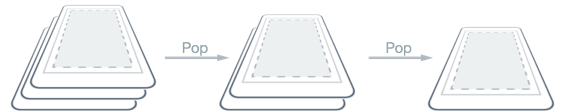
\includegraphics[width=0.75\textwidth]{images/implementation/pop.png}
	\end{center}	
	\caption{Wechsel auf alte Seite}
	\label{fig:pop}
\end{figure}

\paragraph{SignIn Page} stellt die Benutzerschnittstelle zur Anmeldung des Nutzers am System dar, siehe Abbildung \ref{fig:signin}. Dabei gibt dieser die entsprechende IP-Adresse der laufenden Desktopanwendung zur Verbindung an. Durch eine implementierte Logik wird diese IP-Adresse auf ihre Richtigkeit geprüft und die Verbindung gestartet. Bei einer erfolgreichen Verbindung wird der Benutzer zur \gls{app} weitergeleitet, wodurch ihm die entsprechenden Funktionalitäten zur Verfügung stehen. Andernfalls erscheint nach einem definierten Timeout eine Fehlermeldung, welche dem User Informationen vorlegt. Zur Speicherung der IP-Adresse ist zusätzlich die Möglichkeit durch ein Switch Element gegeben, wobei diese bei Start der \gls{app} automatisch eingefügt wird.

\begin{figure}[h]
	\begin{center}
		
\includegraphics[width=0.4\textwidth]{images/implementation/signin.png}
	\end{center}	
	\caption{SignIn Page}
	\label{fig:signin}
\end{figure}

\paragraph{Home Page} stellt die Hauptseite mit der grundlegenden Navigation der \gls{app} dar, indem der Benutzer die Möglichkeit besitzt ein neues Szenario eines Schwarmverhaltens zu starten, Informationen über die \gls{app} abzurufen, oder sich vom aktuelles System abzumelden.

\begin{figure}[h]
	\begin{center}
		
\includegraphics[width=0.4\textwidth]{images/implementation/home.png}
	\end{center}	
	\caption{Home Page}
	\label{fig:home}
\end{figure}

\newpage
\paragraph{Option Page} stellt die Benutzerschnittstelle dar, welche diesen durch die vorhandenen Szenarien anhand eines Carousels leitet und ein entsprechends auswählt.

\begin{figure}[h]
	\begin{center}
		
\includegraphics[width=0.4\textwidth]{images/implementation/option.png}
	\end{center}	
	\caption{Option Page}
	\label{fig:option}
\end{figure}

\newpage
\paragraph{List Page} stellt die Benutzerschnittstelle zur Auswahl der Robotern, welche im Szenario involviert werden sollen. Dabei kann der Benutzer unter den verschiedenen Typen wählen, welche vorhanden sind, wobei die Anzahl der Roboter vom gewählten Szenario abhängt.

\begin{figure}[h]
	\begin{center}
		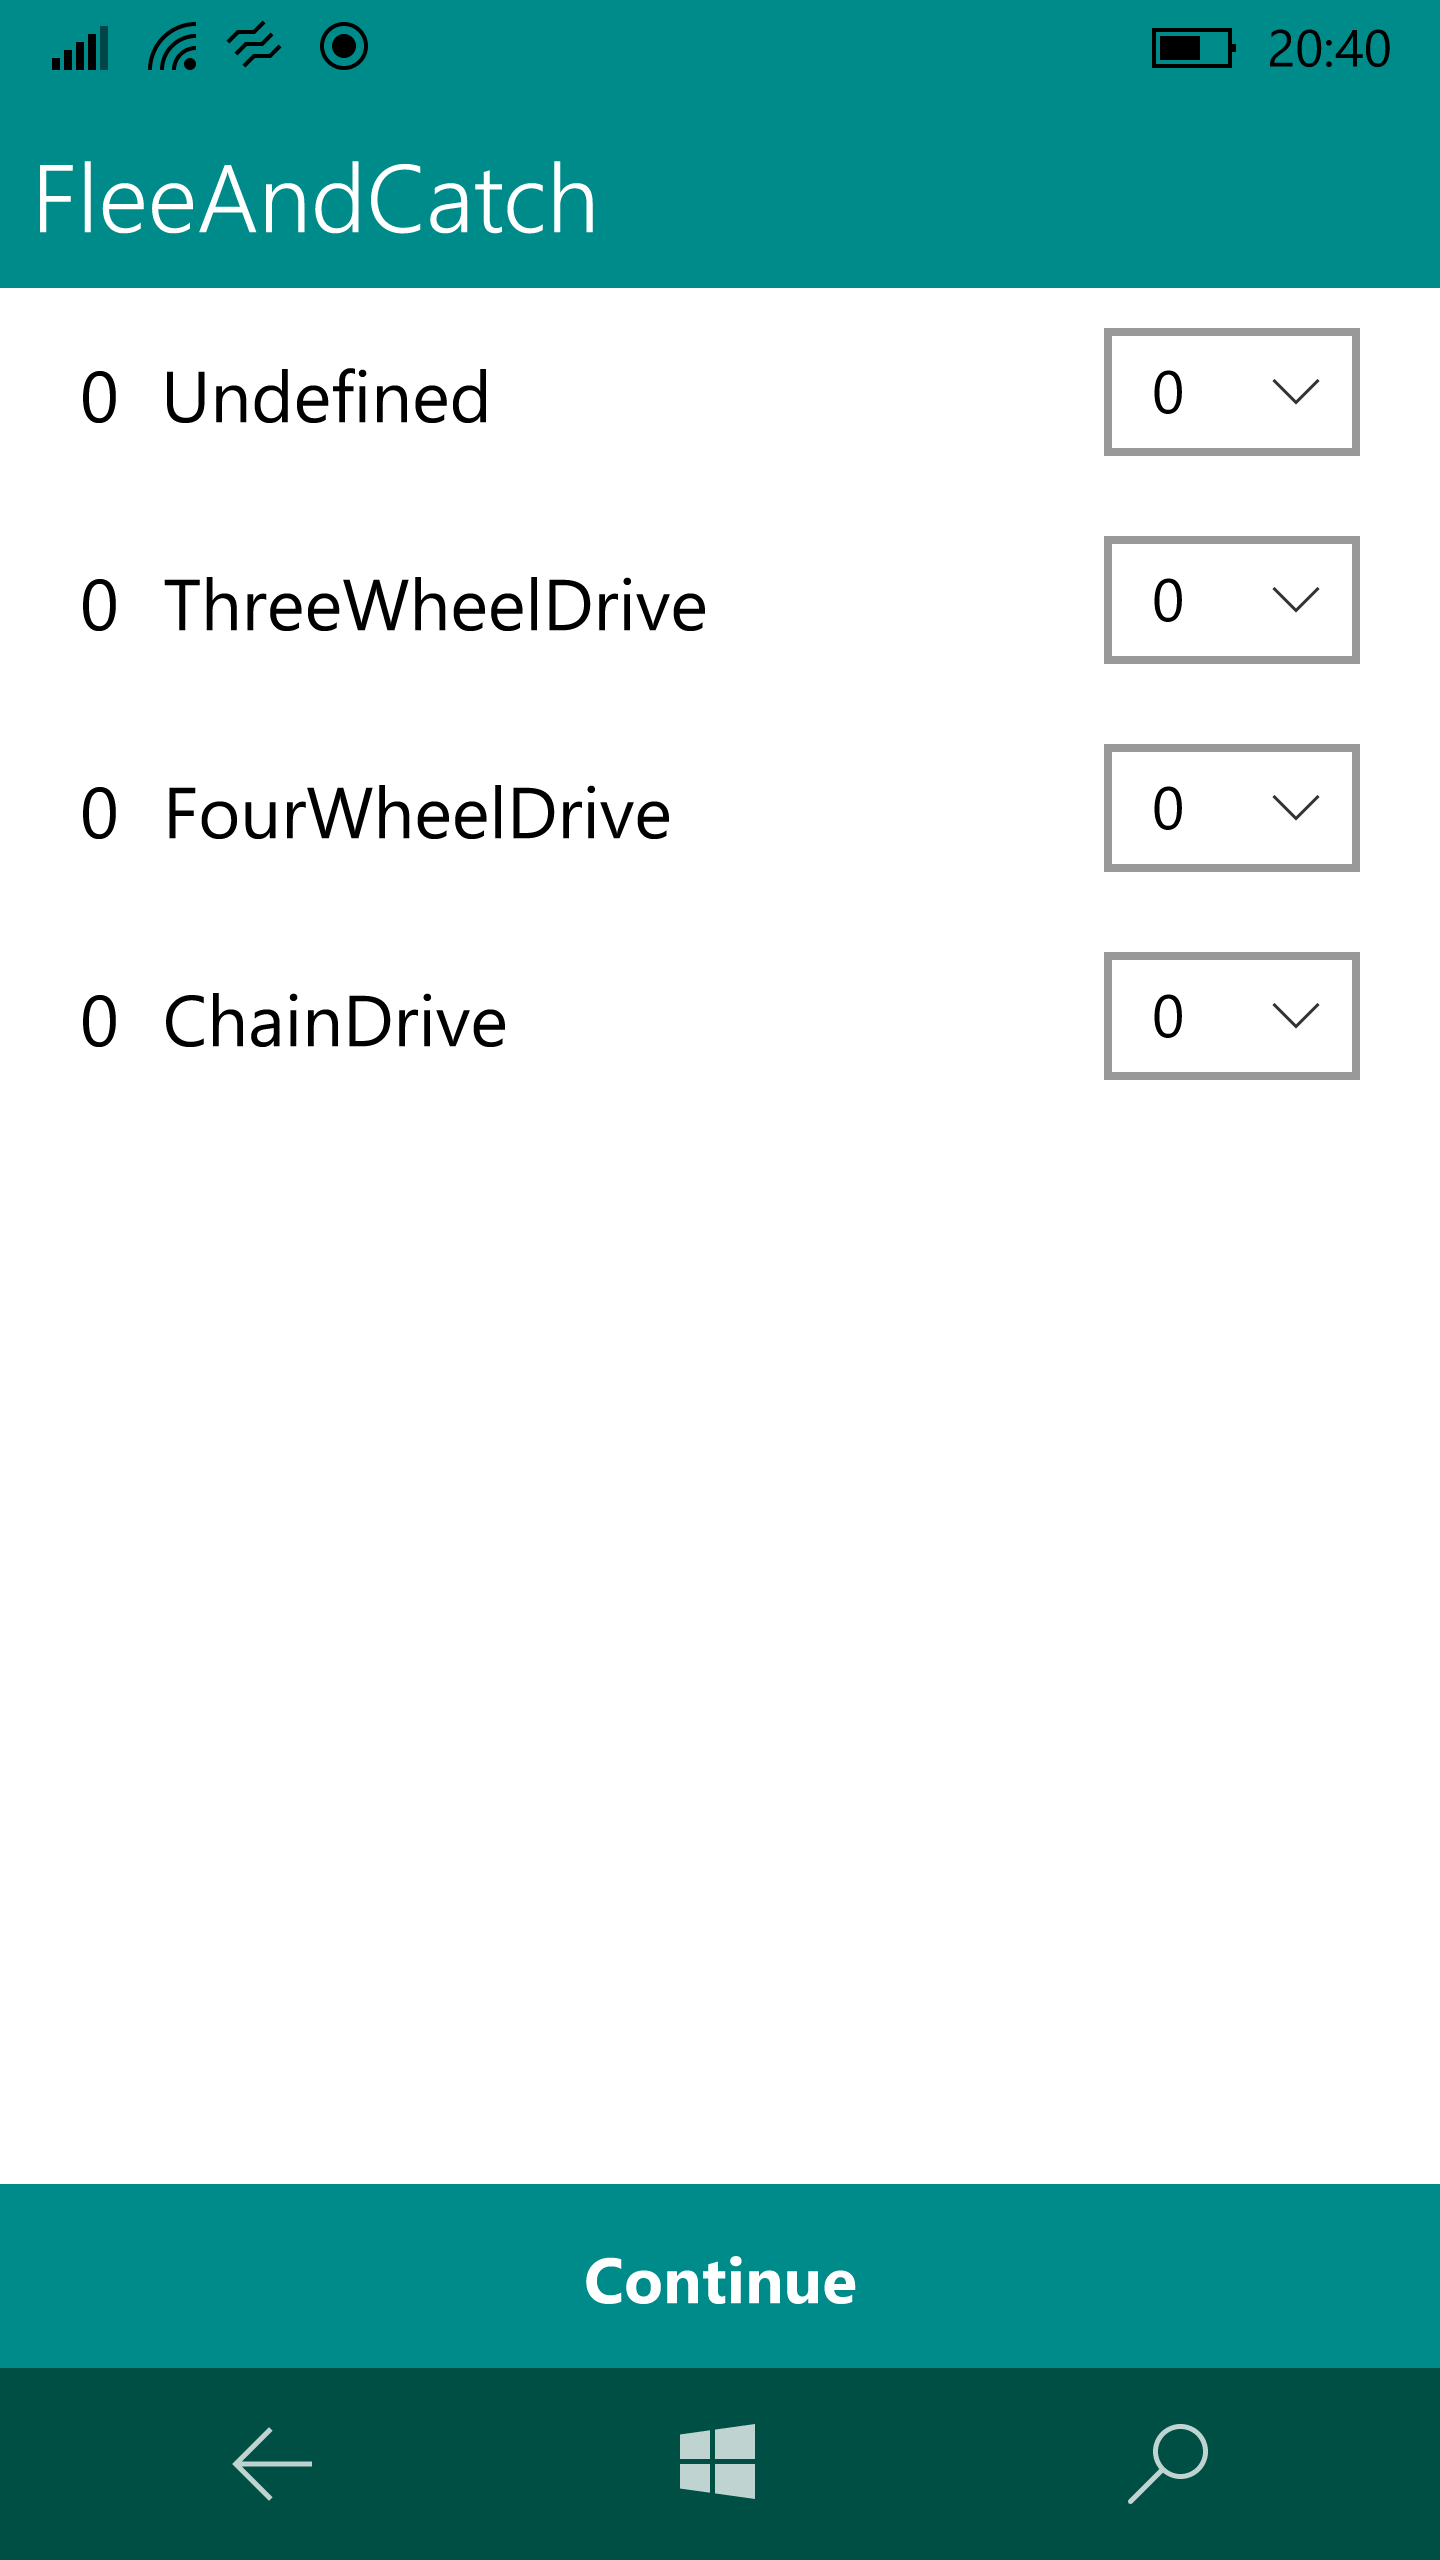
\includegraphics[width=0.4\textwidth]{images/implementation/list.png}
	\end{center}	
	\caption{List Page}
	\label{fig:list}
\end{figure}

\newpage
\paragraph{Szenario Page} stellt die Benutzerschnittselle dar, die einerseits der Steuerung und Überwachung des Schwarmverhaltens dient. Dabei werden laufend die aktuellen Daten der Roboter angezeigt und können durch die Neigungssensoren der eräte gesteuert werden. Diese verhalten sich entsprechend dem ausgewählten SZenario.

\begin{figure}[h]
	\begin{center}
		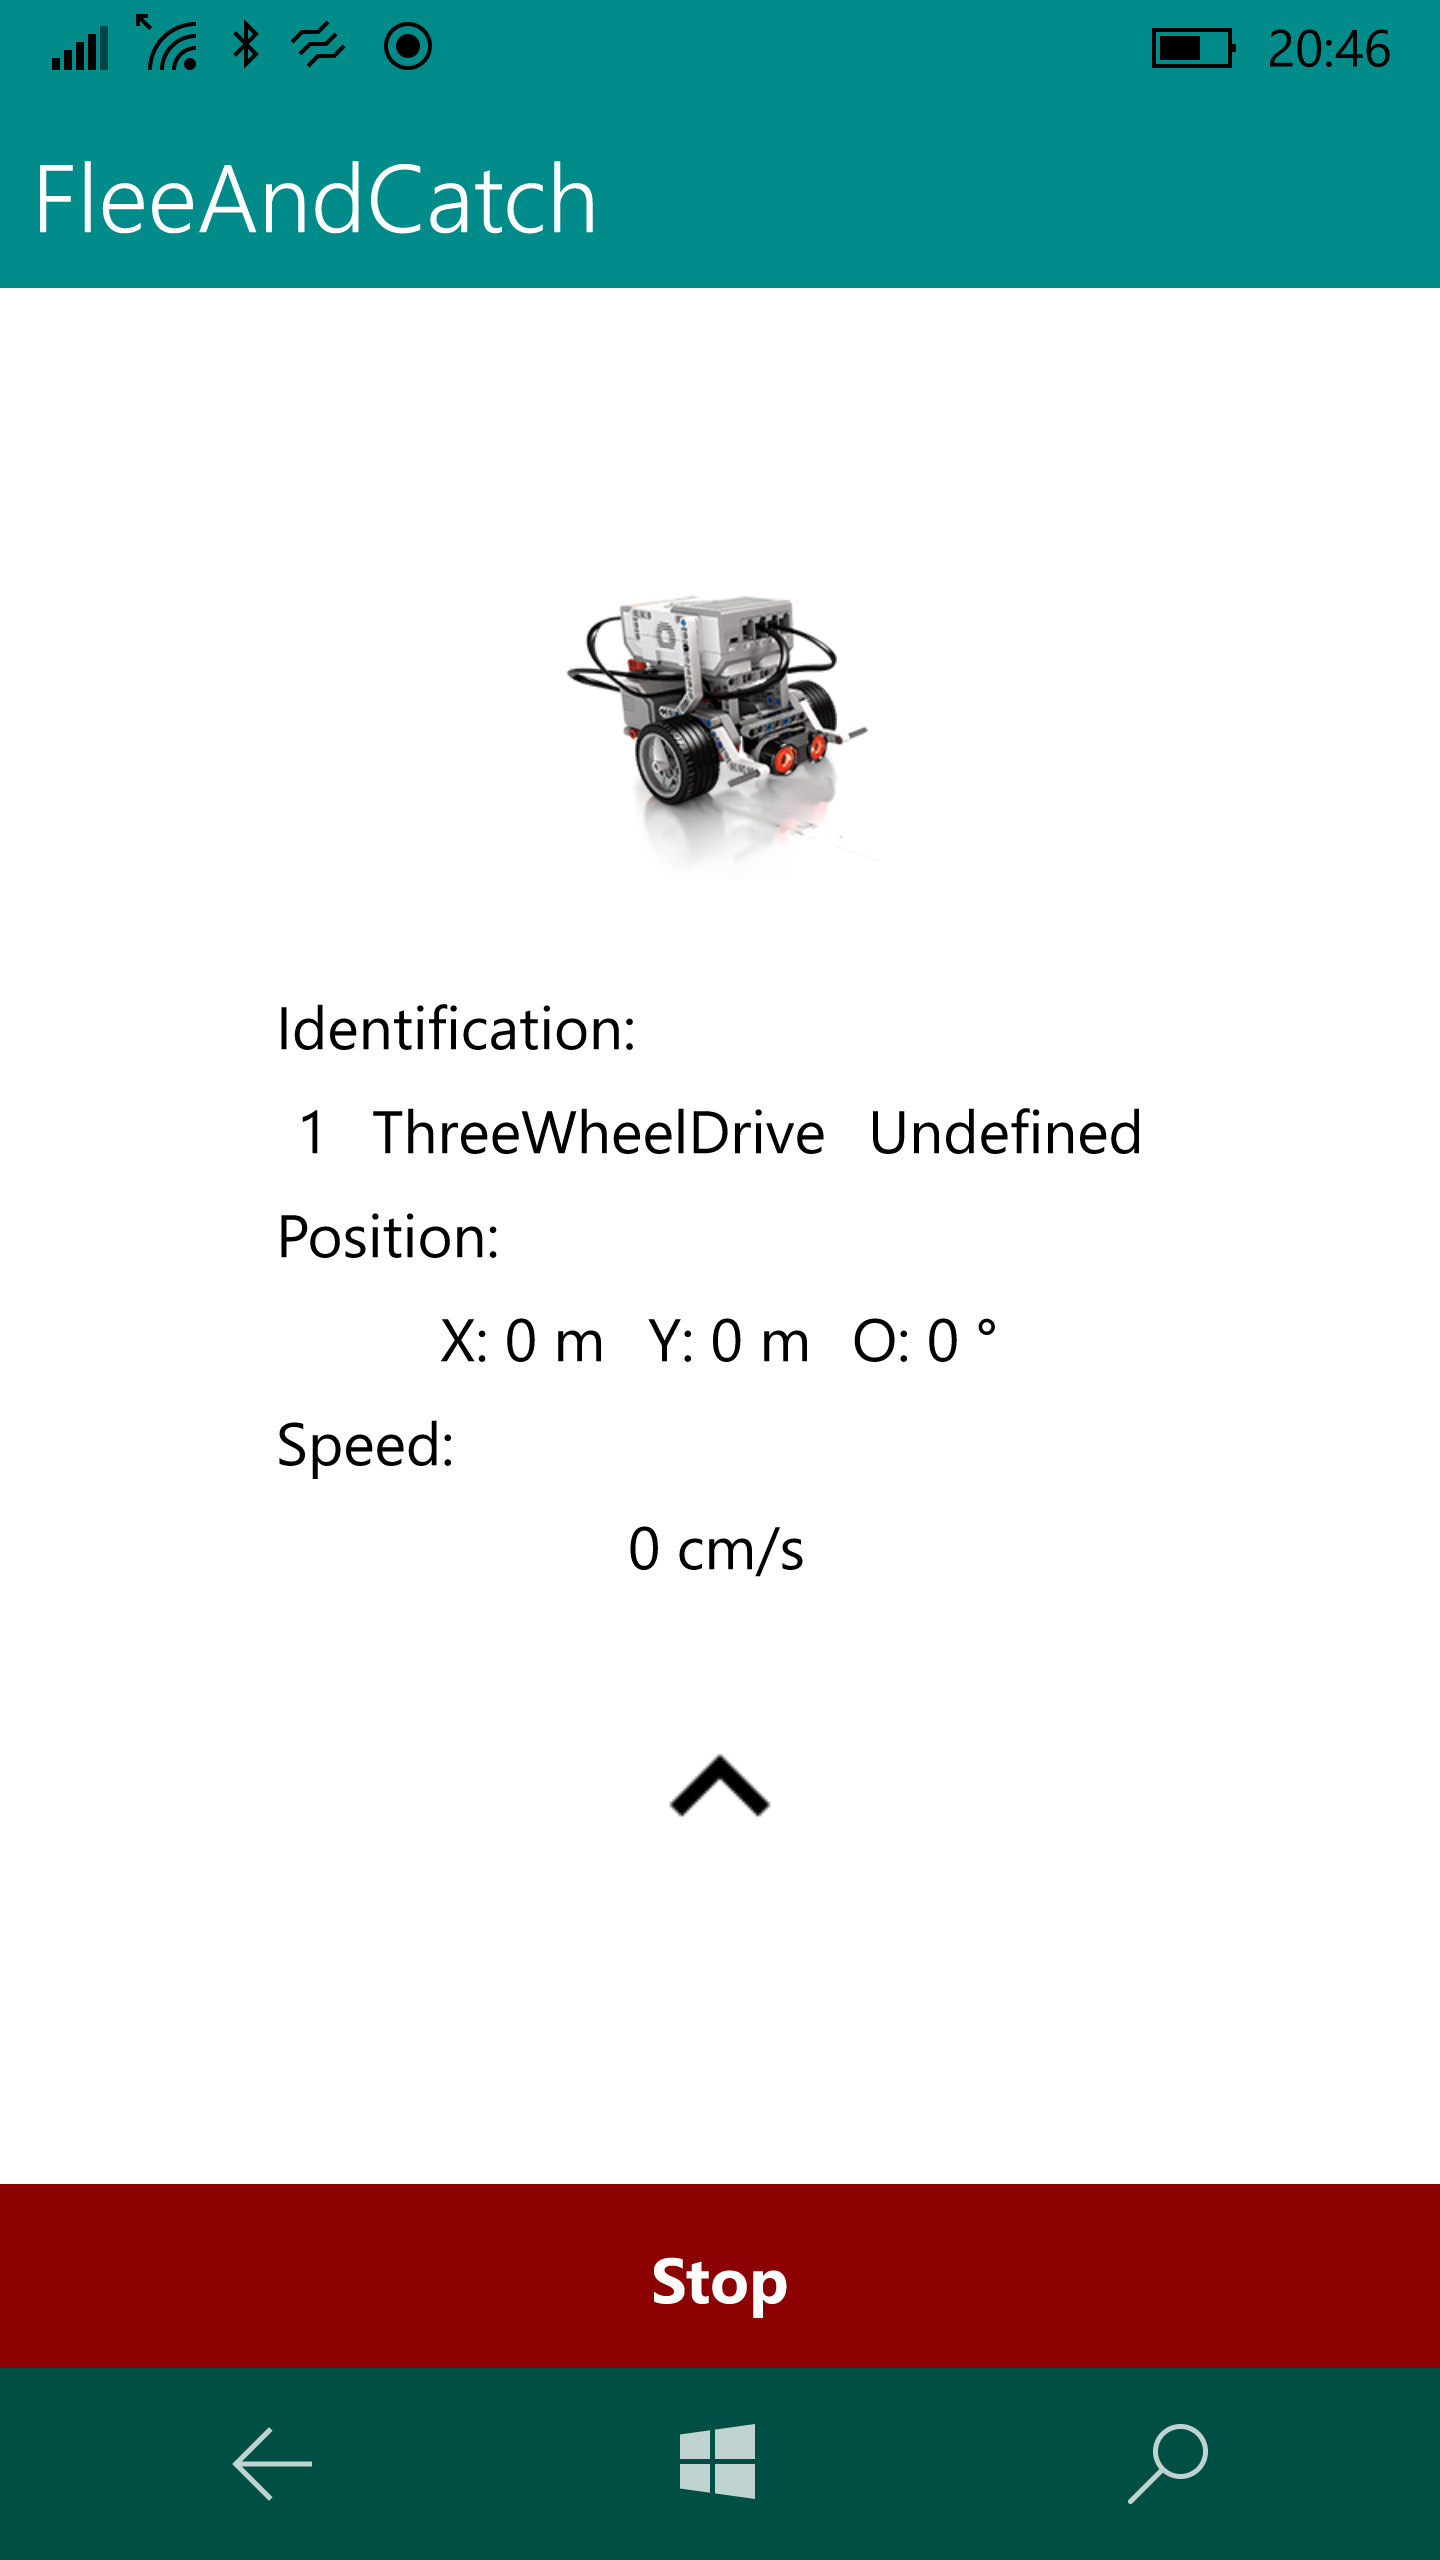
\includegraphics[width=0.4\textwidth]{images/implementation/szenario.png}
	\end{center}	
	\caption{Szenario Page}
	\label{fig:szenario}
\end{figure}

\newpage
\subsubsection{Buisnesslogic} %Logik

\paragraph{Authorization}

\paragraph{Create Szenario}

\paragraph{Szenario}

\newpage
\subsection{Backend}

\begin{comment}
Aufbau
Interpreter
Mechanismen
GUI
\end{comment}

\subsection{Robot}

\begin{comment}
Aufbau
Robot
RobotController
EV3 Library
GUI
\end{comment}